\documentclass[notes,11pt, aspectratio=169]{beamer}

\usepackage{pgfpages}
\setbeameroption{hide notes}

\usepackage{helvet}
\usepackage[default]{lato}
\usepackage{array}
\usepackage{tgbonum}

\usepackage{tikz}
\usepackage{verbatim}
\setbeamertemplate{note page}{\pagecolor{yellow!5}\insertnote}
\usetikzlibrary{positioning}
\usetikzlibrary{calc}
\usetikzlibrary{arrows}
\usetikzlibrary{arrows.meta}
\usetikzlibrary{decorations.markings}
\usetikzlibrary{decorations.pathreplacing}
\usetikzlibrary{shapes.misc}
\usetikzlibrary{shapes.geometric}
\usetikzlibrary{matrix,shapes,arrows,fit,tikzmark}
\usepackage{amsmath}
\usepackage{amssymb}
\usepackage{mathtools}
\usepackage{bm}
\usepackage{mathpazo}
\usepackage{hyperref}
%\usepackage{lipsum}
%\usepackage{multimedia}
\usepackage{graphicx}
\usepackage{multirow}
\usepackage{dcolumn}
%\usepackage{bbm}   % PK-only fonts; not renderable by tectonic (indicator uses \mathbf{1})
\usepackage{pgfplots}
\pgfplotsset{compat=1.18}
\usepackage{listings}
\newcolumntype{d}[0]{D{.}{.}{5}}

\usepackage{changepage}
\usepackage{appendixnumberbeamer}
\newcommand{\beginbackup}{
   \newcounter{framenumbervorappendix}
   \setcounter{framenumbervorappendix}{\value{framenumber}}
   \setbeamertemplate{footline}
   {
     \leavevmode%
     \hline
     box{%
       \begin{beamercolorbox}[wd=\paperwidth,ht=2.25ex,dp=1ex,right]{footlinecolor}%
       \end{beamercolorbox}}%
     \vskip0pt%
   }
 }
\newcommand{\backupend}{
   \addtocounter{framenumbervorappendix}{-\value{framenumber}}
   \addtocounter{framenumber}{\value{framenumbervorappendix}}
}

\usepackage[space]{grffile}
\usepackage{booktabs}
\newcommand\independent{\protect\mathpalette{\protect\independenT}{\perp}}
\def\independenT#1#2{\mathrel{\rlap{$#1#2$}\mkern2mu{#1#2}}}
\DeclareMathOperator{\Supp}{Supp}
\DeclareMathOperator*{\argmin}{arg\,min}
\DeclareMathOperator*{\argmax}{arg\,max}
\DeclareMathOperator{\trace}{trace}
\DeclareMathOperator{\PMI}{PMI}

\definecolor{blue}{RGB}{0,114,178}
\definecolor{red}{RGB}{213,94,0}
\definecolor{yellow}{RGB}{240,228,66}
\definecolor{green}{RGB}{0,158,115}

\hypersetup{
  colorlinks=true,
  linkbordercolor = {white},
  linkcolor = {blue}
}

\definecolor{MyBackground}{RGB}{255,253,218}

\newenvironment{transitionframe}{
  \setbeamercolor{background canvas}{bg=yellow}
  \begin{frame}}{
    \end{frame}
}

\setbeamercolor{frametitle}{fg=blue}
\setbeamercolor{title}{fg=black}
\setbeamertemplate{footline}[frame number]
\setbeamertemplate{navigation symbols}{}
\setbeamertemplate{itemize items}{-}
\setbeamercolor{itemize item}{fg=blue}
\setbeamercolor{itemize subitem}{fg=blue}
\setbeamercolor{enumerate item}{fg=blue}
\setbeamercolor{enumerate subitem}{fg=blue}
\setbeamercolor{button}{bg=MyBackground,fg=blue,}

\setbeamercolor{section in toc}{fg=blue}
\setbeamercolor{subsection in toc}{fg=red}
\setbeamersize{text margin left=1em,text margin right=1em}

\newenvironment{wideitemize}{\itemize\addtolength{\itemsep}{10pt}}{\enditemize}

\lstset{
    language=Python,
    basicstyle=\ttfamily\scriptsize,
    keywordstyle=\color{blue}\bfseries,
    stringstyle=\color{red!70!black},
    commentstyle=\color{green!50!black}\itshape,
    numbers=left,
    numberstyle=\tiny\color{gray},
    numbersep=5pt,
    frame=single,
    breaklines=true,
    backgroundcolor=\color{gray!5},
    showstringspaces=false,
    tabsize=4
}

\newcommand{\va}{\mathbf{a}}
\newcommand{\vc}{\mathbf{c}}
\newcommand{\vd}{\mathbf{d}}
\newcommand{\ve}{\mathbf{e}}
\newcommand{\vh}{\mathbf{h}}
\newcommand{\vp}{\mathbf{p}}
\newcommand{\vu}{\mathbf{u}}
\newcommand{\vv}{\mathbf{v}}
\newcommand{\vw}{\mathbf{w}}
\newcommand{\vx}{\mathbf{x}}
\newcommand{\vy}{\mathbf{y}}
\newcommand{\vz}{\mathbf{z}}
\newcommand{\vq}{\mathbf{q}}
\newcommand{\vk}{\mathbf{k}}
\newcommand{\vA}{\mathbf{A}}
\newcommand{\vB}{\mathbf{B}}
\newcommand{\vE}{\mathbf{E}}
\newcommand{\vM}{\mathbf{M}}
\newcommand{\vU}{\mathbf{U}}
\newcommand{\vV}{\mathbf{V}}
\newcommand{\vW}{\mathbf{W}}
\newcommand{\vX}{\mathbf{X}}
\newcommand{\vY}{\mathbf{Y}}
\newcommand{\vSigma}{\boldsymbol{\Sigma}}
\newcommand{\vLambda}{\boldsymbol{\Lambda}}
\newcommand{\vTheta}{\boldsymbol{\Theta}}
\newcommand{\vphi}{\boldsymbol{\phi}}
\newcommand{\R}{\mathbb{R}}
\newcommand{\E}{\mathbb{E}}
\newcommand{\Frob}{\mathrm{Fro}}


\title[]{\textcolor{blue}{Machine Learning II}\\ \textcolor{black}{\normalsize Lecture 5: Embeddings and Text as Data}}
\author[Quispe]{}
\institute[ENEI]{\small{Alexander Quispe \\ ENEI -- INEI \,\textperiodcentered\, PEU-CD 2026}}
\date{October 19, 2026}


\begin{document}

\begin{frame}[plain]\titlepage\end{frame}

\begin{frame}{Outline}\tableofcontents\end{frame}


\tikzset{
        every picture/.style={remember picture,baseline},
        every node/.style={anchor=base,align=center,outer sep=1.5pt},
        every path/.style={thick},
        }
\tikzstyle{every picture}+=[remember picture]
\tikzstyle{mybox} =[draw=black, very thick, rectangle, inner sep=10pt, inner ysep=20pt]
\tikzstyle{fancytitle} =[draw=black,fill=red, text=white]




% ============================================================
\section{Recap and Motivation}
% ============================================================

\begin{transitionframe}
\begin{center}
{\Huge \textbf{Recap \& Motivation}}\\[10pt]
{\large From latent factors to learned representations}
\end{center}
\end{transitionframe}

\begin{frame}
\frametitle{Where We Left Off}

\textbf{Lecture 6 gave us three viewpoints on the \emph{same} object:}

\vspace{6pt}
\begin{enumerate}
    \item \textbf{SVD / PCA} on a dense matrix $\vX$.
    \item \textbf{Latent factor model} $\vY \approx \vU \vV^\top$ with missing entries.
    \item \textbf{Panel data} with interactive fixed effects (Bai 2009, Athey et al.\ 2021).
\end{enumerate}

\vspace{8pt}
\textbf{The common thread:} each row of $\vU$ is a \emph{vector representation} of a user / unit / entity, and similarity is the dot product $\vu_i^\top \vv_j$.

\vspace{8pt}
\textcolor{red}{Today: these row vectors have a name -- they are \textbf{embeddings} -- and we generalize them well beyond the linear case.}
\end{frame}

\begin{frame}
\frametitle{What Is an Embedding?}

\textbf{Definition.} An embedding is a map
\[
    s \;\longmapsto\; \vu_s \in \R^K
\]
from a discrete object $s$ (a word, song, user, country, firm) to a real-valued vector $\vu_s$.

\vspace{8pt}
\textbf{Two ways to encode meaning:}
\begin{itemize}
    \item \textbf{Distance:} similar objects have similar vectors, $d(\vu_s, \vu_{s'}) = \|\vu_s - \vu_{s'}\|^2$.
    \item \textbf{Inner product:} $d(\vu_s, \vu_{s'}) = \vu_s^\top \vu_{s'}$.
\end{itemize}

\vspace{8pt}
\textbf{Where do the vectors come from?} We \textbf{learn} them from data, by writing down a loss function in which similar objects \emph{should} have similar vectors and letting gradient descent do the work.

\vspace{6pt}
\textcolor{blue}{The embeddings are not specified by the user -- they emerge from the training signal.}
\end{frame}

\begin{frame}
\frametitle{Embedding Examples}

\textbf{The same mathematical object, applied to different domains:}

\vspace{8pt}
\begin{center}
\renewcommand{\arraystretch}{1.4}
\small
\begin{tabular}{p{3cm} p{4.5cm} p{5cm}}
\toprule
\textbf{Domain} & \textbf{Object} & \textbf{Embedding} \\
\midrule
NLP & a word, e.g.\ \textit{king} & $\vv_\text{king} \in \R^{300}$ \\
Recommenders & user $i$, movie $j$ & $\vu_i, \vv_j \in \R^{K}$ \\
Vision & an image & $\vphi(\text{image}) \in \R^{128}$ \\
Multimodal & image + caption & shared $\R^{512}$ (CLIP) \\
Knowledge graphs & entity + relation & $\R^K$ per entity \\
Econ panels (L6) & unit $i$ at time $t$ & $\boldsymbol\lambda_i, \mathbf{F}_t \in \R^K$ \\
\bottomrule
\end{tabular}
\end{center}

\vspace{12pt}
\begin{tikzpicture}
\node [mybox] (box){%
    \begin{minipage}{0.93\textwidth}
    \vspace{-4pt}
    \begin{center}
    \textit{``Good embeddings turn abstract similarity into geometry.''}
    \end{center}
    \end{minipage}
};
\node[fancytitle, right=10pt] at (box.north west) {Takeaway};
\end{tikzpicture}

\vspace{6pt}
\textbf{Why deep learning needs embeddings:} neural nets operate on real-valued vectors, not raw symbolic objects like ``the word \textit{king}'' or ``user \#7''. Embeddings are the bridge from discrete reality to continuous math.
\end{frame}

\begin{frame}
\frametitle{The Narrative Arc}

\begin{center}
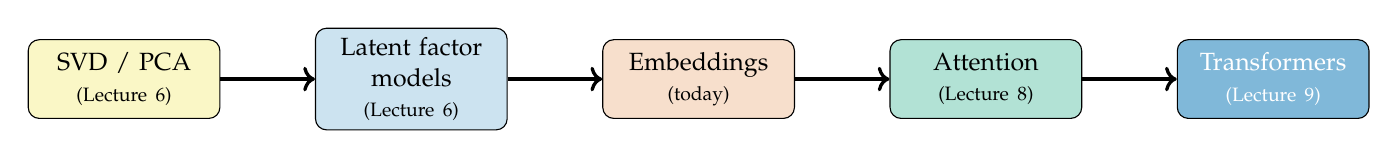
\begin{tikzpicture}[node distance=0.6cm and 1.2cm, every node/.style={draw, rounded corners, align=center, font=\small, minimum height=1cm, text width=2.2cm}]
    \node (svd) [fill=yellow!30] {SVD / PCA \\ \scriptsize (Lecture 6)};
    \node (lfm) [right=of svd, fill=blue!20] {Latent factor models \\ \scriptsize (Lecture 6)};
    \node (emb) [right=of lfm, fill=red!20] {Embeddings \\ \scriptsize (today)};
    \node (att) [right=of emb, fill=green!30] {Attention \\ \scriptsize (Lecture 8)};
    \node (tr)  [right=of att, fill=blue!50, text=white] {Transformers \\ \scriptsize (Lecture 9)};

    \draw[->, very thick] (svd) -- (lfm);
    \draw[->, very thick] (lfm) -- (emb);
    \draw[->, very thick] (emb) -- (att);
    \draw[->, very thick] (att) -- (tr);
\end{tikzpicture}
\end{center}

\vspace{12pt}
\textbf{Reading the arc:}
\begin{itemize}
    \item \textbf{Yesterday:} linear factor models on observed matrices.
    \item \textbf{Today:} learn vector representations of \emph{anything} from co-occurrence data.
    \item \textbf{Next week:} make those representations \emph{context-dependent} (attention).
\end{itemize}

\vspace{6pt}
\textcolor{red}{Each step generalizes the previous one. Same idea, growing expressiveness.}
\end{frame}

\begin{frame}
\frametitle{Why a Whole Lecture on Embeddings?}

\textbf{Embeddings are everywhere in modern ML:}

\vspace{6pt}
\begin{itemize}
    \item Every recommender system: user $\times$ item embeddings.
    \item Every NLP model: word, subword, sentence embeddings.
    \item Every retrieval system: query $\times$ document embeddings.
    \item Every multimodal model: image $\times$ text embeddings (CLIP).
    \item Every knowledge graph: entity $\times$ relation embeddings.
\end{itemize}

\vspace{8pt}
\textbf{And especially for economics:}
\begin{itemize}
    \item Text-as-data: embed FOMC speeches, central bank minutes, news.
    \item Judge / firm / country embeddings from co-occurrence in text or trade.
    \item Embeddings as features for causal inference.
\end{itemize}

\vspace{6pt}
\textcolor{red}{If you understand embeddings, you understand the basic unit of every modern AI system.}
\end{frame}

\begin{frame}
\frametitle{Today's Roadmap (Annotated)}

\begin{enumerate}
    \item \textbf{Manifold learning, briefly.} LLE, t-SNE, UMAP -- dimensionality reduction as a warm-up.
    \item \textbf{Distance vs inner-product embeddings.} Two ways to encode similarity; playlist embedding as a worked example.
    \item \textbf{Word embeddings: word2vec.} Skip-gram, negative sampling, the Levy-Goldberg theorem, classic analogies.
    \item \textbf{Embeddings for economics.} Text-as-data, judge embeddings, firm embeddings, trade.
    \item \textbf{Deep embeddings.} Siamese networks, triplet loss, modern contrastive learning.
    \item \textbf{Static vs contextual.} The limit of word2vec -- and the bridge to Transformers.
\end{enumerate}
\end{frame}


% ============================================================
\section{Manifold Learning, Briefly}
% ============================================================

\begin{transitionframe}
\begin{center}
{\Huge \textbf{Manifold Learning, Briefly}}\\[10pt]
{\large Or: why we need t-SNE and UMAP}
\end{center}
\end{transitionframe}

\begin{frame}
\frametitle{The Manifold Hypothesis}

\textbf{Claim:} high-dimensional data usually lies on (or near) a much lower-dimensional manifold inside the ambient space.

\vspace{8pt}
\textbf{Examples:}
\begin{itemize}
    \item Faces: each $50{,}000$-pixel image is on a $\sim$ 50-dim manifold (pose, expression, lighting).
    \item Text: each one-hot $|V|$-dim word vector lies on a $\sim$ 300-dim ``meaning'' manifold.
    \item Macro time series: a 200-country panel of indicators lies on a low-rank factor manifold.
\end{itemize}

\vspace{8pt}
\textbf{Goal of manifold learning:} find coordinates on that low-dim manifold.

\vspace{6pt}
\textcolor{red}{This is a generalization of PCA: instead of a linear subspace, allow the surface to bend.}
\end{frame}

\begin{frame}
\frametitle{Locally Linear Embedding: Overview}

\textbf{LLE} (Roweis \& Saul, \emph{Science} 2000): the data is \emph{locally} linear even if globally curved.

\vspace{6pt}
\textbf{Two-step recipe:}
\begin{enumerate}
    \item For each point $\vx_i$, find its $B$ nearest neighbors $\mathcal{B}(i)$, and write $\vx_i$ as a convex combination of those neighbors. This produces a weight matrix $\vW$ that captures \emph{local geometry}.

    \vspace{4pt}
    \item Find low-dim points $\vu_i$ that satisfy the \emph{same} reconstruction weights.
\end{enumerate}

\vspace{12pt}
\begin{tikzpicture}
\node [mybox] (box){%
    \begin{minipage}{0.93\textwidth}
    \vspace{-4pt}
    \begin{center}
    \textbf{Key idea:} learn $\vW$ from high-dim data, then transfer it to low dim.
    \end{center}
    \end{minipage}
};
\node[fancytitle, right=10pt] at (box.north west) {Local reconstruction};
\end{tikzpicture}

\vspace{8pt}
We now unpack each of the two steps in detail.
\end{frame}

\begin{frame}
\frametitle{LLE Step 1: Local Reconstruction Weights}

\textbf{Given:} $n$ high-dim points $\vx_1, \ldots, \vx_n$ and neighborhoods $\mathcal{B}(i)$.

\vspace{6pt}
\textbf{For each point $\vx_i$,} solve a small local problem:
\[
    \min_{W_{i,*}} \;\Bigl\| \vx_i - \sum_{j \in \mathcal{B}(i)} W_{ij}\, \vx_j \Bigr\|^2
    \quad \text{s.t.\ } \sum_{j \in \mathcal{B}(i)} W_{ij} = 1.
\]

\vspace{6pt}
\textbf{Concrete example.} If $\mathcal{B}(i) = \{3, 17, 22\}$, then
\[
    \vx_i \approx W_{i,3}\, \vx_3 + W_{i,17}\, \vx_{17} + W_{i,22}\, \vx_{22}
\]
with $W_{i,3} + W_{i,17} + W_{i,22} = 1$.

\vspace{8pt}
\textbf{Storage.} The full weight matrix $\vW$ is $n \times n$ but \textbf{sparse} -- row $i$ has at most $B$ nonzero entries.

\vspace{4pt}
\textit{If $n = 100$ and $B = 5$, we solve 100 small problems, each with 5 unknowns.}
\end{frame}

\begin{frame}
\frametitle{LLE Step 1: The Algebraic Trick}

\textbf{Use the constraint} $\sum_j W_{ij} = 1$ to rewrite the residual:
\[
    \vx_i - \sum_j W_{ij}\, \vx_j
    \;=\; \sum_j W_{ij}\, (\vx_i - \vx_j).
\]

\vspace{6pt}
\textbf{Squared norm} expands as a quadratic form:
\[
    \Bigl\| \sum_j W_{ij} (\vx_i - \vx_j) \Bigr\|^2
    \;=\; \sum_{j, k} W_{ij} W_{ik}\, C^i_{jk}
\]
where
\[
    C^i_{jk} = (\vx_i - \vx_j)^\top (\vx_i - \vx_k).
\]

\vspace{8pt}
\textbf{Interpretation.} $C^i$ is the \emph{local Gram matrix} (covariance of neighbor offsets around $\vx_i$).

\vspace{6pt}
\textbf{Closed form.} Each row $W_{i,*}$ is found by solving a small linear system with $C^i$ on the left-hand side -- $B$ variables, one Lagrange multiplier for the sum-to-one constraint. No iteration needed.
\end{frame}

\begin{frame}
\frametitle{LLE Step 2: Learn the Low-Dim Embedding}

\textbf{Keep $\vW$ fixed.} Now search for low-dim coordinates $\vu_i \in \R^K$ that satisfy the \emph{same} reconstruction:
\[
    \argmin_{\vU} \;\sum_i \Bigl\| \vu_i - \sum_{j \in \mathcal{B}(i)} W_{ij}\, \vu_j \Bigr\|^2.
\]

\vspace{6pt}
\textbf{Interpretation.} ``If $\vx_i$ was a convex combination of its neighbors in high dim, the same convex combination should reproduce $\vu_i$ in low dim.'' This preserves \emph{local geometry}.

\vspace{8pt}
\textbf{Trivial solution issue.} Without constraints, $\vU = 0$ minimizes the objective. So we add:
\[
    \sum_i \vu_i = 0 \quad\text{(centering)}, \qquad
    \tfrac{1}{n} \vU^\top \vU = \mathbf{I}_K \quad\text{(unit variance per axis)}.
\]

\vspace{4pt}
\textit{Notation convention used here:} $\vU \in \R^{n \times K}$ with one row per point.
\end{frame}

\begin{frame}
\frametitle{LLE Step 2: A Small Numerical Example}

\textbf{Setup.} Three collinear points in 2D, project to $K = 1$:
\[
    \vx_1 = (0, 0), \quad \vx_2 = (1, 1), \quad \vx_3 = (2, 2).
\]

\vspace{4pt}
\textbf{Step 1 (already done).} For $\vx_2$ with neighbors $\{\vx_1, \vx_3\}$, solving the local problem gives
\[
    W_{2,1} = 0.5, \quad W_{2,3} = 0.5
    \quad\text{(since $\vx_2 = 0.5\,\vx_1 + 0.5\,\vx_3$)}.
\]

\vspace{4pt}
\textbf{Step 2.} Find scalars $u_1, u_2, u_3 \in \R$ that satisfy the \emph{same} reconstruction:
\[
    u_2 \;=\; 0.5\,u_1 + 0.5\,u_3.
\]

\vspace{4pt}
\textbf{Apply the constraints.}

\vspace{2pt}
Centering: $u_1 + u_2 + u_3 = 0$. Substituting $u_2 = 0.5(u_1 + u_3)$:
\[
    1.5(u_1 + u_3) = 0 \;\Rightarrow\; u_3 = -u_1, \;\; u_2 = 0.
\]

Unit variance: $\tfrac{1}{3}(u_1^2 + u_2^2 + u_3^2) = 1$. With $u_3 = -u_1$ and $u_2 = 0$:
\[
    \tfrac{2u_1^2}{3} = 1 \;\Rightarrow\; u_1 = -\sqrt{1.5} \approx -1.22.
\]
\end{frame}

\begin{frame}
\frametitle{LLE Step 2: Interpretation of the Numerical Example}

\textbf{Recovered 1D embedding:}
\[
    (u_1, u_2, u_3) \;=\; \bigl(-\sqrt{1.5},\;\; 0,\;\; \sqrt{1.5}\bigr) \approx (-1.22,\; 0,\; 1.22).
\]

\vspace{8pt}
\begin{center}
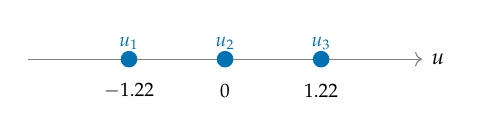
\begin{tikzpicture}[scale=1.0]
    \draw[->, gray] (-2.5, 0) -- (2.5, 0) node[right, black] {\footnotesize $u$};
    \foreach \x in {-1.22, 0, 1.22} {
        \draw[gray] (\x, -0.1) -- (\x, 0.1);
    }

    \fill[blue] (-1.22, 0) circle (3pt) node[above] {\scriptsize $u_1$};
    \fill[blue] (0, 0) circle (3pt) node[above] {\scriptsize $u_2$};
    \fill[blue] (1.22, 0) circle (3pt) node[above] {\scriptsize $u_3$};

    \node[font=\scriptsize] at (-1.22, -0.4) {$-1.22$};
    \node[font=\scriptsize] at (0, -0.4) {$0$};
    \node[font=\scriptsize] at (1.22, -0.4) {$1.22$};
\end{tikzpicture}
\end{center}

\vspace{6pt}
\textbf{What the algorithm achieved:}
\begin{itemize}
    \item The three points lie on a 1D line in 2D; LLE found that line.
    \item The \emph{ordering} along the line is preserved: $u_1 < u_2 < u_3$.
    \item The \emph{local reconstruction} holds: $u_2 = 0.5\,u_1 + 0.5\,u_3 = 0$.
    \item The sign is arbitrary -- $(+\sqrt{1.5}, 0, -\sqrt{1.5})$ is equally valid.
\end{itemize}

\vspace{6pt}
\textcolor{red}{Same algorithm, scaled up.} For thousands of points, we solve this via an eigendecomposition (next slide) instead of hand-calculating constraints.
\end{frame}

\begin{frame}
\frametitle{LLE Step 2: Matrix Form and Eigendecomposition}

\textbf{Define} $\vA = \mathbf{I}_n - \vW$. The objective becomes:
\[
    \sum_i \Bigl\| \vu_i - \sum_j W_{ij}\, \vu_j \Bigr\|^2
    \;=\; \|\vA \vU\|_\Frob^2
    \;=\; \trace(\vU^\top \vA^\top \vA \vU).
\]

\vspace{6pt}
\textbf{Let} $\vM = \vA^\top \vA = (\mathbf{I}_n - \vW)^\top (\mathbf{I}_n - \vW)$.

\vspace{6pt}
\textbf{Entrywise:}
\[
    M_{ij} = \mathbf{1}_{[i=j]} - W_{ij} - W_{ji} + \sum_k W_{ki} W_{kj}.
\]

\vspace{6pt}
\textbf{Properties of $\vM$:}
\begin{itemize}
    \item Symmetric: $\vM = \vM^\top$.
    \item Positive semidefinite: $\vz^\top \vM \vz = \|\vA \vz\|^2 \geq 0$ for any $\vz$.
\end{itemize}

\vspace{6pt}
\textbf{Solution} (min-max theorem applied to $\trace(\vU^\top \vM \vU)$ s.t. orthonormality): $\vU$ = bottom $K$ \emph{non-trivial} eigenvectors of $\vM$ (skipping the zero eigenvalue from $\vM \mathbf{1} = 0$).

\vspace{4pt}
\textcolor{red}{$\vM$ penalizes low-dim embeddings that break the local reconstruction encoded by $\vW$.}
\end{frame}

\begin{frame}
\frametitle{Section Summary}

\textbf{Manifold learning:} find low-dim coordinates that preserve geometric structure.

\vspace{6pt}
\textbf{LLE} (Roweis \& Saul, \emph{Science} 2000) is the canonical example:
\begin{itemize}
    \item \textbf{Step 1.} Learn local weights $\vW$ that reconstruct each point from its neighbors.
    \item \textbf{Step 2.} Find low-dim points $\vU$ that satisfy the \emph{same} reconstruction. \\
    Solution: bottom $K$ non-trivial eigenvectors of $\vM = (\mathbf{I} - \vW)^\top(\mathbf{I} - \vW)$.
\end{itemize}

\vspace{8pt}
\textbf{Related modern tools} (t-SNE, UMAP) follow the same template -- preserve a notion of locality between high- and low-dim representations -- but use different loss functions.

\vspace{8pt}
\textcolor{red}{Critical caveat:} manifold-learning outputs are \textbf{visualizations}. The 2D pictures they produce should never be used as features for a downstream model.

\vspace{6pt}
\textbf{Coming up:} the embeddings we \emph{do} use as features are learned from a different objective -- not preserving distances, but predicting co-occurrence in sequences.
\end{frame}


% ============================================================
\section{Distance vs Inner-Product Embeddings}
% ============================================================

\begin{transitionframe}
\begin{center}
{\Huge \textbf{Distance vs Inner-Product Embeddings}}\\[10pt]
{\large Two geometries, two interpretations}
\end{center}
\end{transitionframe}

\begin{frame}
\frametitle{Two Ways to Encode Similarity}

\textbf{Distance-based:}
\[
    P(s \mid s') \propto \exp\bigl(-\|\vu_s - \vu_{s'}\|^2\bigr)
\]
Two objects are similar if their vectors are close in Euclidean distance.

\vspace{8pt}
\textbf{Inner-product based:}
\[
    P(s \mid s') \propto \exp\bigl(\vu_s^\top \vv_{s'}\bigr)
\]
Two objects are similar if their vectors point in similar directions.

\vspace{8pt}
\textbf{They produce very different geometries:}
\begin{itemize}
    \item Distance $\to$ clustering: objects of the same ``type'' form tight clouds.
    \item Inner product $\to$ direction: meaning is encoded by orientation, magnitude can vary.
\end{itemize}

\vspace{4pt}
\textcolor{blue}{Inner product is exactly the latent factor model from Lecture 6.}
\end{frame}

\begin{frame}
\frametitle{Two Geometries, Side by Side}

\begin{columns}[T]
\begin{column}{0.5\textwidth}
\centering
\textbf{Distance-based}

\vspace{4pt}
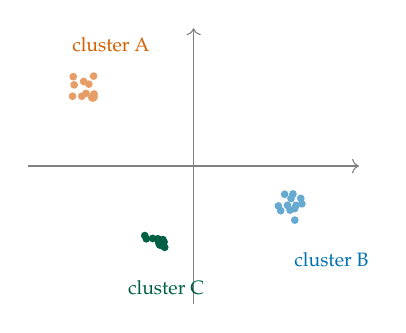
\begin{tikzpicture}[scale=0.7]
    \draw[->, gray, thin] (-3, 0) -- (3, 0);
    \draw[->, gray, thin] (0, -2.5) -- (0, 2.5);

    \foreach \i in {1,...,12} {
        \pgfmathsetmacro{\x}{-2.2 + 0.4*rnd}
        \pgfmathsetmacro{\y}{1.2 + 0.5*rnd}
        \fill[red!60] (\x, \y) circle (2pt);
    }
    \node[red] at (-1.5, 2.2) {\scriptsize cluster A};

    \foreach \i in {1,...,12} {
        \pgfmathsetmacro{\x}{1.5 + 0.5*rnd}
        \pgfmathsetmacro{\y}{-1 + 0.6*rnd}
        \fill[blue!60] (\x, \y) circle (2pt);
    }
    \node[blue] at (2.5, -1.7) {\scriptsize cluster B};

    \foreach \i in {1,...,12} {
        \pgfmathsetmacro{\x}{-1 + 0.5*rnd}
        \pgfmathsetmacro{\y}{-1.5 + 0.4*rnd}
        \fill[green!60!black] (\x, \y) circle (2pt);
    }
    \node[green!60!black] at (-0.5, -2.2) {\scriptsize cluster C};
\end{tikzpicture}

\vspace{4pt}
{\small Clusters in space.}
\end{column}

\begin{column}{0.5\textwidth}
\centering
\textbf{Inner-product based}

\vspace{4pt}
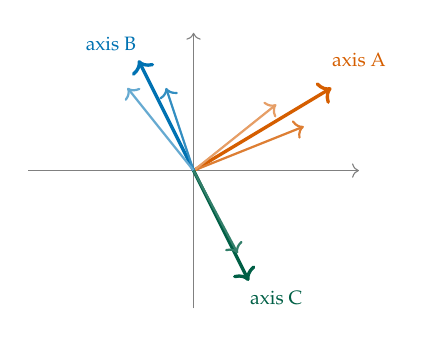
\begin{tikzpicture}[scale=0.7]
    \draw[->, gray, thin] (-3, 0) -- (3, 0);
    \draw[->, gray, thin] (0, -2.5) -- (0, 2.5);

    \draw[->, red, very thick] (0,0) -- (2.5, 1.5);
    \draw[->, red!80, thick] (0,0) -- (2, 0.8);
    \draw[->, red!60, thick] (0,0) -- (1.5, 1.2);
    \node[red] at (3, 2) {\scriptsize axis A};

    \draw[->, blue, very thick] (0,0) -- (-1, 2);
    \draw[->, blue!80, thick] (0,0) -- (-0.5, 1.5);
    \draw[->, blue!60, thick] (0,0) -- (-1.2, 1.5);
    \node[blue] at (-1.5, 2.3) {\scriptsize axis B};

    \draw[->, green!60!black, very thick] (0,0) -- (1, -2);
    \draw[->, green!60!black!80, thick] (0,0) -- (0.8, -1.5);
    \node[green!60!black] at (1.5, -2.3) {\scriptsize axis C};
\end{tikzpicture}

\vspace{4pt}
{\small Directions, varying magnitudes.}
\end{column}
\end{columns}

\vspace{12pt}
\textbf{Use distance when:} objects have a natural notion of locality (songs near other songs of similar genre).

\textbf{Use inner product when:} you want \emph{compositionality} -- $\vu_a + \vu_b \approx \vu_c$ makes sense.
\end{frame}

\begin{frame}
\frametitle{Inner Product = Latent Factor Model}

\textbf{Recall from Lecture 6:}
\[
    Y_{ij} \approx \vu_i^\top \vv_j
\]
where $\vu_i$ is a user vector and $\vv_j$ is an item vector.

\vspace{8pt}
\textbf{Embedding view:} $\vU$ contains one row per user, $\vV$ contains one row per item. The dot product gives a similarity score.

\vspace{8pt}
\textbf{To convert to a probabilistic model:}
\[
    P(\text{item } s \mid \text{user } s') = \frac{\exp(\vu_s^\top \vv_{s'})}{\sum_{s''} \exp(\vu_{s''}^\top \vv_{s'})}
\]

\vspace{4pt}
The softmax form lets us train via maximum likelihood instead of squared error.

\vspace{6pt}
\textcolor{red}{Same vectors, different loss. The geometry is shaped by what we minimize.}
\end{frame}

\begin{frame}
\frametitle{Worked Example: Playlist Embeddings}

\textbf{Setup} (Chen et al., 2012): Spotify-style playlist data, sequences of songs.

\vspace{4pt}
\textbf{Model:} for each song $s$, an entry vector $\vu_s$ and an exit vector $\vv_s$.
\[
    P(s \mid s') = \frac{\exp(-\|\vu_s - \vv_{s'}\|^2)}{\sum_{s''} \exp(-\|\vu_{s''} - \vv_{s'}\|^2)}
\]

\vspace{4pt}
\textbf{Parameters:} $2K|S|$ -- linear in vocabulary, not quadratic.

\vspace{8pt}
\textbf{Training:} maximize the log-likelihood of observed playlists,
\[
    \argmax_{\vU, \vV} \sum_{\text{playlists}} \sum_{j} \log P\bigl(p_i^j \mid p_i^{j-1}\bigr).
\]

\vspace{6pt}
\textbf{Simpler ``single-point'' variant:} use $\vu_s$ for both roles. Less expressive but easier to visualize.

\vspace{4pt}
\textcolor{blue}{Same mathematical structure will reappear in word2vec.}
\end{frame}

\begin{frame}
\frametitle{The Cold-Start Problem}

\textbf{What happens when a new song / item arrives?}
\begin{itemize}
    \item No co-occurrence data yet, so no signal to learn $\vu_s$.
    \item Default to $\vu_s = 0$ or random: both are bad.
\end{itemize}

\vspace{8pt}
\textbf{Solution: side information.} If the new song has tags (genre, artist, year), learn an embedding of tags as well:
\[
    \vu_s \approx \frac{1}{|T_s|} \sum_{t \in T_s} \va_t
\]
where $\va_t$ is the tag embedding.

\vspace{8pt}
\textbf{Generalization} (key idea for what's coming):
\begin{itemize}
    \item Without side info $\to$ embedding looked up by ID (matrix factorization).
    \item With side info $\to$ embedding \emph{computed} from features.
\end{itemize}

\vspace{4pt}
\textcolor{red}{The cold-start fix is the seed of every two-tower retrieval and deep embedding model.}
\end{frame}


% ============================================================
\section{Word Embeddings: word2vec}
% ============================================================

\begin{transitionframe}
\begin{center}
{\Huge \textbf{Word Embeddings: word2vec}}\\[10pt]
{\large The canonical embedding}
\end{center}
\end{transitionframe}

\begin{frame}
\frametitle{From Geometric to Sequence-Based Embeddings}

\textbf{Where we were:}
\begin{itemize}
    \item \textbf{LLE} (and t-SNE / UMAP): preserve \emph{local geometry}. The training signal is ``which points were close in high dim?''
\end{itemize}

\vspace{6pt}
\textbf{Where we're going:}
\begin{itemize}
    \item \textbf{word2vec}: preserve \emph{co-occurrence in sequences}. The training signal is ``which words appeared next to each other?''
\end{itemize}

\vspace{8pt}
\textbf{Same machinery, different signal.} Both produce vectors; only the training data differs.

\vspace{8pt}
\textbf{Concrete example.} Consider three sentences:
\begin{itemize}
    \item ``the dog jumped over the fence''
    \item ``my dog ate my homework''
    \item ``I walked my dog up to the fence''
\end{itemize}

\vspace{4pt}
The word \textit{dog} appears near \textit{jumped, ate, walked, fence, the, my, over}. \\
These context co-occurrences are the training signal for $\vv_\text{dog}$.

\vspace{4pt}
\textcolor{red}{Distributional semantics:} ``a word is known by the company it keeps.''
\end{frame}

\begin{frame}
\frametitle{The Distributional Hypothesis}

\begin{tikzpicture}
\node [mybox] (box){%
    \begin{minipage}{0.93\textwidth}
    \vspace{-4pt}
    \begin{center}
    \textit{``You shall know a word by the company it keeps.''} \\[2pt]
    \small -- J. R. Firth (1957)
    \end{center}
    \end{minipage}
};
\node[fancytitle, right=10pt] at (box.north west) {Linguistic principle};
\end{tikzpicture}

\vspace{12pt}
\textbf{Implication:} we can learn the meaning of a word from the distribution of words around it.

\vspace{6pt}
\textbf{Example.} Consider:
\begin{itemize}
    \item ``The Federal Reserve \emph{raised} interest rates.''
    \item ``The central bank \emph{lifted} its policy rate.''
    \item ``The Fed \emph{hiked} the benchmark.''
\end{itemize}

\vspace{4pt}
\textit{Raised}, \textit{lifted}, \textit{hiked} appear in very similar contexts $\to$ they should have similar embeddings.

\vspace{6pt}
\textcolor{red}{Word2vec operationalizes this hypothesis as a learning objective.}
\end{frame}

\begin{frame}
\frametitle{Why Probability Tables Don't Work}

\textbf{Naive model:} a giant table of bigram probabilities $P(w \mid w')$.

\vspace{8pt}
\textbf{For a vocabulary of $|V|$ words:}
\begin{center}
\renewcommand{\arraystretch}{1.2}
\begin{tabular}{ll}
\toprule
\textbf{$|V|$} & \textbf{\# table entries $|V|^2$} \\
\midrule
$10{,}000$ (small) & $10^8$ \\
$100{,}000$ (typical English) & $10^{10}$ \\
$1{,}000{,}000$ (Spanish + named entities) & $10^{12}$ \\
\bottomrule
\end{tabular}
\end{center}

\vspace{8pt}
\textbf{And it gets worse:} most $(w, w')$ pairs are never observed, so the model can't generalize.

\vspace{8pt}
\textbf{Embedding solution:} represent each word as a $K$-dim vector with $K \sim 100$. Total parameters: $K|V|$ -- linear, not quadratic.

\vspace{4pt}
\textcolor{red}{Generalization comes from shared structure: words with similar embeddings transfer information.}
\end{frame}

\begin{frame}
\frametitle{Skip-Gram Model: The Objective}

\textbf{Skip-gram} (Mikolov, Sutskever, Chen, Corrado, Dean, NIPS 2013): for each word in the corpus, predict the words in its context.

\vspace{6pt}
\begin{center}
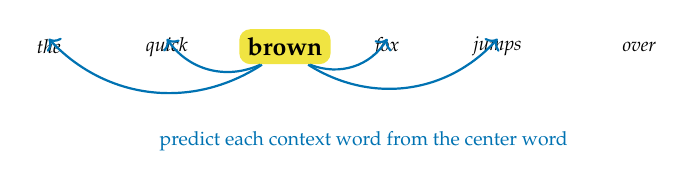
\begin{tikzpicture}[scale=1.0]
    \node[font=\scriptsize] at (-4, 0) {\textit{the}};
    \node[font=\scriptsize] at (-2.5, 0) {\textit{quick}};
    \node[font=\small, fill=yellow, rounded corners, inner sep=3pt] (c) at (-1, 0) {\textbf{brown}};
    \node[font=\scriptsize] at (0.3, 0) {\textit{fox}};
    \node[font=\scriptsize] at (1.7, 0) {\textit{jumps}};
    \node[font=\scriptsize] at (3.5, 0) {\textit{over}};

    \draw[->, blue, thick] (c) to[bend left=40] (-2.5, 0.1);
    \draw[->, blue, thick] (c) to[bend left=40] (-4, 0.1);
    \draw[->, blue, thick] (c) to[bend right=40] (0.3, 0.1);
    \draw[->, blue, thick] (c) to[bend right=40] (1.7, 0.1);

    \node[font=\scriptsize, blue] at (0, -1.2) {predict each context word from the center word};
\end{tikzpicture}
\end{center}

\vspace{6pt}
\textbf{Notation conventions for this section:}
\begin{itemize}
    \item Vocabulary $S = \{s_1, \ldots, s_W\}$, size $W$. Embedding dimension $D$.
    \item Corpus is a sequence $w_1, w_2, \ldots, w_T$ of tokens from $S$.
    \item $w_I$ = center / input word. $w_O$ = output / context word.
    \item $\vv_w \in \R^D$ = \textbf{input} embedding (when $w$ is the center).
    \item $\vv'_w \in \R^D$ = \textbf{output} embedding (when $w$ is the context).
\end{itemize}

\vspace{6pt}
\textbf{Objective} for window size $s$ over corpus length $T$:
\[
    \argmax_{\vV, \vV'} \;\frac{1}{T} \sum_{t=1}^T \sum_{\substack{-s \leq j \leq s \\ j \neq 0}} \log P\bigl(w_{t+j} \mid w_t\bigr).
\]

\vspace{4pt}
\textbf{Conditional probability:}
\[
    P(w_O \mid w_I) = \frac{\exp\!\bigl(\vv'^{\,\top}_{w_O}\, \vv_{w_I}\bigr)}
                           {\sum_{w \in S} \exp\!\bigl(\vv'^{\,\top}_{w}\, \vv_{w_I}\bigr)}.
\]

\vspace{4pt}
\textcolor{red}{$j = 0$ excluded: predicting a word from itself is trivial.}
\end{frame}

\begin{frame}
\frametitle{Skip-Gram: A Concrete Example}

\textbf{Sentence.} \hspace{6pt} ``the dog jumped over the fence''

\vspace{4pt}
\textbf{Indexing.}
\[
    w_1 = \text{the}, \;\; w_2 = \text{dog}, \;\; w_3 = \text{jumped}, \;\; w_4 = \text{over}, \;\; w_5 = \text{the}, \;\; w_6 = \text{fence}.
\]

\vspace{6pt}
\textbf{Window size $s = 2$, center $w_2 = \textit{dog}$.} Context words are $w_1, w_3, w_4$.

\vspace{6pt}
\textbf{Training pairs (center, context):}
\begin{center}
\renewcommand{\arraystretch}{1.2}
\small
\begin{tabular}{lll}
\toprule
\textbf{Pair} & \textbf{Use vectors} & \textbf{Score} \\
\midrule
$(\text{dog}, \text{the})$ & $\vv_\text{dog}$, $\vv'_\text{the}$ & $\vv'^{\,\top}_\text{the}\,\vv_\text{dog}$ \\
$(\text{dog}, \text{jumped})$ & $\vv_\text{dog}$, $\vv'_\text{jumped}$ & $\vv'^{\,\top}_\text{jumped}\,\vv_\text{dog}$ \\
$(\text{dog}, \text{over})$ & $\vv_\text{dog}$, $\vv'_\text{over}$ & $\vv'^{\,\top}_\text{over}\,\vv_\text{dog}$ \\
\bottomrule
\end{tabular}
\end{center}

\vspace{6pt}
\textbf{Then slide the window:} $w_3 = \textit{jumped}$ becomes the new center, and we generate new pairs $(\textit{jumped}, w_1), (\textit{jumped}, w_2), (\textit{jumped}, w_4), (\textit{jumped}, w_5)$.

\vspace{4pt}
\textcolor{blue}{This pair-generation step is the entire training data preparation for word2vec.}
\end{frame}

\begin{frame}
\frametitle{Why Two Vectors Per Word?}

\textbf{Each word $w$ gets two embeddings:}
\begin{itemize}
    \item $\vv_w \in \R^D$: used when $w$ plays the role of \textbf{input / center}.
    \item $\vv'_w \in \R^D$: used when $w$ plays the role of \textbf{output / context}.
\end{itemize}

\vspace{8pt}
\textbf{Score for the pair $(w_I, w_O)$:}
\[
    \text{score}(w_I, w_O) \;=\; \vv'^{\,\top}_{w_O}\, \vv_{w_I}.
\]

\vspace{6pt}
\textbf{Example.} For pair $(\text{dog}, \text{jumped})$:
\[
    \text{score} = \vv'^{\,\top}_\text{jumped}\, \vv_\text{dog}.
\]

\vspace{8pt}
\textbf{Why two?}
\begin{itemize}
    \item Separates the two roles cleanly; the math becomes asymmetric in the right way.
    \item Empirically gives better embeddings than tying $\vv_w = \vv'_w$.
\end{itemize}

\textbf{Final embedding.} After training, most people keep $\vv_w$ (or sometimes $\tfrac{1}{2}(\vv_w + \vv'_w)$).

\vspace{4pt}
\textcolor{blue}{Implementation:} two \texttt{nn.Embedding} layers of size $W \times D$ each.
\end{frame}

\begin{frame}
\frametitle{The Softmax Denominator Problem}

\textbf{The probability:}
\[
    P(w_O \mid w_I) = \frac{\exp\!\bigl(\vv'^{\,\top}_{w_O}\, \vv_{w_I}\bigr)}
                           {\underbrace{\sum_{w \in S} \exp\!\bigl(\vv'^{\,\top}_{w}\, \vv_{w_I}\bigr)}_{Z(w_I)}}
\]

\vspace{6pt}
\textbf{Bad news:} computing the denominator requires summing over the entire vocabulary -- $|V| \sim 10^5$ or $10^6$ words.

\vspace{4pt}
\textbf{Worse:} we do this for every training example, every gradient step.

\vspace{8pt}
\textbf{Two solutions in the original paper:}
\begin{enumerate}
    \item \textcolor{red}{Negative sampling} -- approximate the softmax by sampling. (The modern standard.)
    \item Hierarchical softmax -- replace the $W$-way softmax by a binary tree of depth $\log_2 W$.
\end{enumerate}

\vspace{4pt}
We treat them in that order. But first, let's make the softmax concrete with numbers.
\end{frame}

\begin{frame}
\frametitle{Softmax: A Numerical Example}

\textbf{Tiny vocabulary} $S = \{\text{dog}, \text{jumped}, \text{pizza}\}$, $W = 3$, $D = 2$.

\vspace{4pt}
\textbf{Input embedding of the center word:}
\[
    \vv_\text{dog} = \begin{bmatrix} 1 \\ 2 \end{bmatrix}.
\]

\vspace{4pt}
\textbf{Output embeddings of every possible context:}
\[
    \vv'_\text{dog} = \begin{bmatrix} 0 \\ 1 \end{bmatrix}, \quad
    \vv'_\text{jumped} = \begin{bmatrix} 2 \\ 1 \end{bmatrix}, \quad
    \vv'_\text{pizza} = \begin{bmatrix} -1 \\ 0 \end{bmatrix}.
\]

\vspace{6pt}
\textbf{Compute the three scores:}
\begin{align*}
    \text{score}(\text{dog}) &= \vv'^{\,\top}_\text{dog}\, \vv_\text{dog} = 0\cdot 1 + 1\cdot 2 = 2, \\
    \text{score}(\text{jumped}) &= \vv'^{\,\top}_\text{jumped}\, \vv_\text{dog} = 2\cdot 1 + 1\cdot 2 = 4, \\
    \text{score}(\text{pizza}) &= \vv'^{\,\top}_\text{pizza}\, \vv_\text{dog} = -1\cdot 1 + 0\cdot 2 = -1.
\end{align*}
\end{frame}

\begin{frame}
\frametitle{Softmax Numerical Example: The Probabilities}

\textbf{Exponentiate and normalize:}
\begin{align*}
    e^{2} &\approx 7.39, & e^{4} &\approx 54.60, & e^{-1} &\approx 0.37. \\
    Z &= 7.39 + 54.60 + 0.37 \approx 62.36.
\end{align*}

\vspace{6pt}
\textbf{Softmax probabilities:}
\[
    P(\text{jumped} \mid \text{dog}) = \frac{54.60}{62.36} \approx 0.875.
\]
\[
    P(\text{dog} \mid \text{dog}) = \frac{7.39}{62.36} \approx 0.118, \quad
    P(\text{pizza} \mid \text{dog}) = \frac{0.37}{62.36} \approx 0.006.
\]

\vspace{8pt}
\begin{tikzpicture}
\node [mybox] (box){%
    \begin{minipage}{0.93\textwidth}
    \vspace{-4pt}
    The model thinks ``\textit{jumped}'' is the likely context of ``\textit{dog}'' because the dot product $\vv'^{\,\top}_\text{jumped}\, \vv_\text{dog}$ is large.
    \end{minipage}
};
\node[fancytitle, right=10pt] at (box.north west) {Interpretation};
\end{tikzpicture}

\vspace{4pt}
\textcolor{red}{Training pushes the score of the \emph{actual} observed context up, and competing scores down.}
\end{frame}

\begin{frame}
\frametitle{Training Word2vec by Gradient Descent}

\textbf{Negative log-likelihood:}
\[
    \min_{\vV, \vV'} \;
    \underbrace{\sum_{t=1}^T \sum_{\substack{-s \leq j \leq s \\ j \neq 0}}}_{\text{all (center, context) pairs}}
    \;\bigl[ -\log P\bigl(w_{t+j} \mid w_t\bigr) \bigr].
\]

\vspace{6pt}
\textbf{Reading the loss:}
\begin{itemize}
    \item Observed pair $(w_t, w_{t+j})$ should have \emph{high} probability $\to$ \emph{low} $-\log P$.
    \item Unobserved (random) pairs implicitly carry weight through the denominator.
\end{itemize}

\vspace{8pt}
\textbf{What gradient descent does:}
\begin{enumerate}
    \item Increases $\vv'^{\,\top}_{w_{t+j}}\, \vv_{w_t}$ for real (center, context) pairs.
    \item Decreases $\vv'^{\,\top}_{w}\, \vv_{w_t}$ for all other vocabulary words $w$.
\end{enumerate}

\vspace{4pt}
\textbf{Initialization.} Random; SGD or Adam with mini-batches over pairs.
\end{frame}

\begin{frame}
\frametitle{Why Full Softmax Is Expensive}

\textbf{Big-O recap.} ``Cost is $O(f(n))$'' means the work grows like $f(n)$ as $n$ grows, ignoring constants.

\vspace{6pt}
\textbf{The softmax denominator:}
\[
    Z(w_I) = \sum_{w=1}^W \exp\!\bigl(\vv'^{\,\top}_w\, \vv_{w_I}\bigr).
\]

\vspace{4pt}
\textbf{Cost analysis:}
\begin{itemize}
    \item $W$ dot products.
    \item Each dot product touches $D$ coordinates.
    \item Total: $O(W D)$ per training pair.
\end{itemize}

\vspace{6pt}
\textbf{Concrete example.} $W = 100{,}000$, $D = 300$:
\[
    W \cdot D = 30{,}000{,}000 \;\text{coordinate operations per pair}.
\]

With billions of training pairs in a corpus, this is unworkable.

\vspace{6pt}
\textcolor{red}{Note:} a careful implementation computes \emph{all} $P(w \mid w_I)$ in one pass over the vocabulary -- $O(WD)$, not $O(W^2 D)$. Naive code can accidentally do the $W^2$ version.
\end{frame}

\begin{frame}
\frametitle{Gradient of the Log-Softmax}

\textbf{Goal:} compute $\nabla_{\vv_{w_I}} \log P(w_O \mid w_I)$ for SGD.

\vspace{6pt}
\textbf{Start from:}
\[
    \log P(w_O \mid w_I)
    = \vv'^{\,\top}_{w_O}\, \vv_{w_I} \;-\; \log Z(w_I)
\]
where $Z(w_I) = \sum_w \exp(\vv'^{\,\top}_w\, \vv_{w_I})$.

\vspace{6pt}
\textbf{Derivative of the first term:}
\[
    \nabla_{\vv_{w_I}} \bigl(\vv'^{\,\top}_{w_O}\, \vv_{w_I}\bigr) = \vv'_{w_O}.
\]

\textbf{Derivative of the log-partition (chain rule):}
\[
    \nabla_{\vv_{w_I}} \log Z(w_I)
    = \frac{1}{Z} \sum_w \exp\!\bigl(\vv'^{\,\top}_w\, \vv_{w_I}\bigr)\, \vv'_w
    = \sum_w P(w \mid w_I)\, \vv'_w.
\]

\textbf{Combining:}
\[
    \boxed{\;\nabla_{\vv_{w_I}} \log P(w_O \mid w_I)
    = \vv'_{w_O} \;-\; \sum_{w=1}^W P(w \mid w_I)\, \vv'_w\;}
\]

\vspace{4pt}
\textcolor{red}{Move $\vv_{w_I}$ toward the true context $\vv'_{w_O}$ and away from the model's average prediction.}
\end{frame}

\begin{frame}
\frametitle{Negative Sampling}

\textbf{Idea:} replace the softmax classification (``which word among $W$?'') with many binary classifications (``is this pair real or fake?'').

\vspace{8pt}
\textbf{For each observed pair $(w_I, w_O)$:}
\begin{itemize}
    \item Treat $(w_I, w_O)$ as a \textbf{positive} example: real co-occurrence.
    \item Sample $k$ words $\tilde w_1, \ldots, \tilde w_k$ from a noise distribution $q$.
    \item Treat $(w_I, \tilde w_i)$ as \textbf{negative} examples: random.
\end{itemize}

\vspace{8pt}
\textbf{Loss for one $(w_I, w_O)$ pair:}
\[
    \mathcal{L} = -\log \sigma\!\bigl(\vv'^{\,\top}_{w_O}\, \vv_{w_I}\bigr)
        \;-\; \sum_{i=1}^k \log \sigma\!\bigl(-\vv'^{\,\top}_{\tilde w_i}\, \vv_{w_I}\bigr)
\]
where $\sigma$ is the sigmoid.

\vspace{4pt}
\textbf{Per step cost:} $O(k D)$ instead of $O(W D)$. Typically $k = 5$ to $20$.

\vspace{4pt}
\textcolor{red}{This is the actual word2vec training procedure used in practice.}
\end{frame}

\begin{frame}
\frametitle{Why Hierarchical Softmax?}

\textbf{Regular softmax} asks one big question:
\[
    \text{``Among all $W$ vocabulary words, which is the context?''}
\]
Cost: $O(W D)$.

\vspace{8pt}
\textbf{Hierarchical softmax} replaces it with a sequence of binary questions:
\[
    \text{``Go left or right?''} \;\to\; \text{``Go left or right?''} \;\to\; \cdots
\]
until reaching the target leaf.

\vspace{8pt}
\textbf{Setup.}
\begin{itemize}
    \item Build a \emph{binary tree} whose \textbf{leaves} are the $W$ vocabulary words.
    \item Each \textbf{internal node} (including the root) has its own embedding vector. \\
    Internal nodes are \emph{not} words -- they are decision points.
\end{itemize}

\vspace{6pt}
\textbf{Cost per training pair:} $O(L D)$ where $L$ is the path length to the target leaf. For a balanced tree, $L = \log_2 W$.

\vspace{4pt}
\textcolor{red}{For $W = 10^5$: $\log_2 W \approx 17$. We replace 100{,}000 dot products with 17.}
\end{frame}

\begin{frame}
\frametitle{Hierarchical Softmax: The Math}

\textbf{Small example tree:}

\vspace{2pt}
\begin{center}
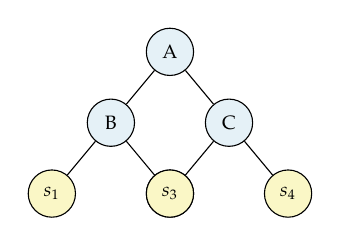
\begin{tikzpicture}[level distance=0.9cm, sibling distance=1.5cm,
    every node/.style={draw, circle, fill=blue!10, minimum size=0.6cm, font=\scriptsize}]
    \node {A}
        child {node {B}
            child {node[fill=yellow!30] {$s_1$}}
            child {node[fill=yellow!30] {$s_2$}}
        }
        child {node {C}
            child {node[fill=yellow!30] {$s_3$}}
            child {node[fill=yellow!30] {$s_4$}}
        };
\end{tikzpicture}
\end{center}

\textbf{Each internal node has a vector} $\va_\text{node} \in \R^D$ (learned).

\vspace{4pt}
\textbf{At each node, branching probability uses a sigmoid:}
\[
    P(\text{left} \mid w_I) = \sigma\!\bigl(\va_\text{node}^\top\, \vv_{w_I}\bigr),
    \qquad
    P(\text{right} \mid w_I) = 1 - \sigma(\cdot).
\]

\textbf{Probability of a leaf} = product along its path. Example:
\[
    P(s_3 \mid w_I) = P(\text{right at A}) \cdot P(\text{left at C}).
\]

\vspace{4pt}
\textcolor{blue}{Training:} same gradient descent objective. The path probabilities replace the softmax denominator.
\end{frame}

\begin{frame}
\frametitle{Hierarchical Softmax: Cost Comparison}

\renewcommand{\arraystretch}{1.3}
\begin{center}
\small
\begin{tabular}{l c c c}
\toprule
\textbf{Method} & \textbf{Cost per pair} & \textbf{$W = 10^4$, $D = 100$} & \textbf{$W = 10^5$, $D = 300$} \\
\midrule
Full softmax & $O(W D)$ & $10^6$ & $3 \cdot 10^7$ \\
Hierarchical softmax & $O(\log_2(W) \cdot D)$ & $\approx 1{,}300$ & $\approx 5{,}100$ \\
Negative sampling & $O(k D)$ & $\approx 1{,}000$ & $\approx 3{,}000$ \\
\bottomrule
\end{tabular}
\end{center}

\vspace{8pt}
\textbf{Takeaways:}
\begin{itemize}
    \item Both tricks scale; full softmax does not.
    \item Negative sampling and hierarchical softmax are comparable in cost.
    \item Modern systems prefer negative sampling: simpler, more parallel, fewer hyperparameters.
\end{itemize}

\vspace{8pt}
\textcolor{red}{Hierarchical softmax still matters when:} you need exact probabilities (negative sampling only approximates), or you're working on tasks where the tree structure is meaningful (e.g., the WordNet hierarchy).
\end{frame}

\begin{frame}
\frametitle{Why Huffman Trees?}

\textbf{Observation:} cost is proportional to \emph{path length} to the target leaf.

\vspace{4pt}
If a word appears \textbf{often}, its leaf is visited often. We want it to have a \textbf{short path}.

\vspace{8pt}
\textbf{Huffman coding} (1952): given word frequencies, build the tree that minimizes the \emph{expected path length}
\[
    \mathbb{E}[L] = \sum_w f_w \cdot L_w
\]
where $f_w$ is the frequency of word $w$ and $L_w$ is its path length.

\vspace{8pt}
\textbf{Two contrasting cases:}
\begin{itemize}
    \item \textbf{All words equally frequent} $\to$ balanced tree is optimal; every leaf has depth $\log_2 W$.
    \item \textbf{Very skewed frequencies} (typical for language: Zipf's law) $\to$ Huffman tree is much better.
\end{itemize}

\vspace{6pt}
\textcolor{blue}{For word2vec, English Wikipedia has Zipfian frequencies. Huffman gives big speedups.}
\end{frame}

\begin{frame}
\frametitle{Huffman Construction: How It Works}

\textbf{Algorithm.}
\begin{enumerate}
    \item Treat each word as a leaf with weight = frequency.
    \item Find the two smallest-weight nodes; merge them into a new node whose weight is the sum.
    \item Repeat until one node (the root) remains.
\end{enumerate}

\vspace{6pt}
\textbf{Worked example.} Suppose we have these word frequencies:
\[
    f_\text{do} = 18, \;\; f_\text{you} = 4, \;\; f_\text{know} = 7, \;\; f_\text{the} = 20,
\]
\[
    f_\text{way} = 9, \;\; f_\text{of} = 4, \;\; f_\text{devil} = 5, \;\; f_\text{queen} = 6.
\]

\vspace{6pt}
\textbf{Merging steps} (always combine the two smallest):
\begin{enumerate}
    \item $\text{you}(4) + \text{of}(4) = 8$
    \item $\text{devil}(5) + \text{queen}(6) = 11$
    \item $\text{know}(7) + 8 = 15$
    \item $\text{way}(9) + 11 = 20$
    \item $15 + \text{do}(18) = 33$
    \item $\text{the}(20) + 20 = 40$
    \item $33 + 40 = 73 \;\to\; \text{root}$
\end{enumerate}
\end{frame}

\begin{frame}
\frametitle{Huffman Example: Expected Path Length}

\textbf{Resulting Huffman path lengths} (one valid assignment):
\vspace{4pt}
\begin{center}
\renewcommand{\arraystretch}{1.2}
\small
\begin{tabular}{l c c c}
\toprule
\textbf{Word} & \textbf{Frequency $f_w$} & \textbf{Huffman path length $L_w$} & \textbf{$f_w \cdot L_w$} \\
\midrule
do & 18 & 2 & 36 \\
the & 20 & 2 & 40 \\
know & 7 & 3 & 21 \\
way & 9 & 3 & 27 \\
you & 4 & 4 & 16 \\
of & 4 & 4 & 16 \\
devil & 5 & 4 & 20 \\
queen & 6 & 4 & 24 \\
\midrule
\textbf{Total} & \textbf{73} & & \textbf{200} \\
\bottomrule
\end{tabular}
\end{center}

\vspace{6pt}
\textbf{Expected Huffman path length:} $\mathbb{E}[L]_\text{Huffman} = 200 / 73 \approx 2.74$.

\vspace{4pt}
\textbf{Balanced binary tree with 8 words:} every leaf at depth 3, so $\mathbb{E}[L]_\text{balanced} = 3$.

\vspace{6pt}
\begin{tikzpicture}
\node [mybox] (box){%
    \begin{minipage}{0.93\textwidth}
    \vspace{-4pt}
    Huffman is about \textbf{9\% cheaper} on average here. On real Zipfian corpora, the savings are much larger.
    \end{minipage}
};
\node[fancytitle, right=10pt] at (box.north west) {Why Huffman beats balanced};
\end{tikzpicture}
\end{frame}

\begin{frame}
\frametitle{Vector Arithmetic in Embedding Space}

\textbf{The famous result:}
\[
    \vv_{\text{king}} - \vv_{\text{man}} + \vv_{\text{woman}} \;\approx\; \vv_{\text{queen}}
\]

\vspace{8pt}
\begin{center}
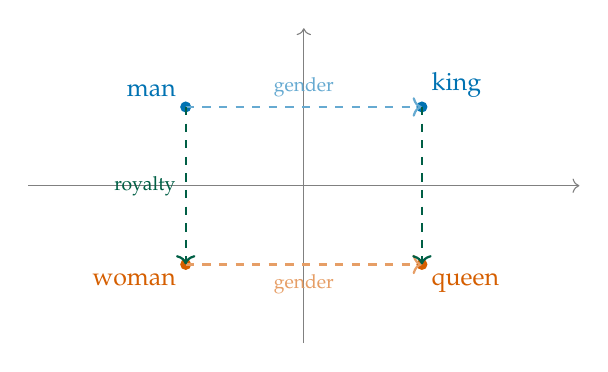
\begin{tikzpicture}[scale=1.0]
    \draw[->, gray, thin] (-3.5, 0) -- (3.5, 0);
    \draw[->, gray, thin] (0, -2) -- (0, 2);

    \fill[blue] (-1.5, 1) circle (2pt) node[above left, font=\small] {man};
    \fill[blue] (1.5, 1) circle (2pt) node[above right, font=\small] {king};
    \fill[red] (-1.5, -1) circle (2pt) node[below left, font=\small] {woman};
    \fill[red] (1.5, -1) circle (2pt) node[below right, font=\small] {queen};

    \draw[->, blue!60, thick, dashed] (-1.5, 1) -- (1.5, 1) node[midway, above, font=\scriptsize] {gender};
    \draw[->, red!60, thick, dashed] (-1.5, -1) -- (1.5, -1) node[midway, below, font=\scriptsize] {gender};

    \draw[->, green!60!black, thick, dashed] (-1.5, 1) -- (-1.5, -1) node[midway, left, font=\scriptsize] {royalty};
    \draw[->, green!60!black, thick, dashed] (1.5, 1) -- (1.5, -1);
\end{tikzpicture}
\end{center}

\vspace{8pt}
\textbf{Geometric reading:} ``gender'' and ``royalty'' are nearly orthogonal directions, so the parallelogram closes.

\vspace{6pt}
\textcolor{red}{This is not magic.} It is a direct consequence of the linear structure of the PMI matrix.
\end{frame}

\begin{frame}
\frametitle{Examples From the Original Paper}

\textbf{Mikolov et al.\ (2013) found these analogies hold:}

\vspace{4pt}
\begin{center}
\renewcommand{\arraystretch}{1.3}
\small
\begin{tabular}{l l l l}
\toprule
\textbf{Relationship} & \textbf{Example 1} & \textbf{Example 2} & \textbf{Example 3} \\
\midrule
country : capital & France : Paris & Japan : Tokyo & Italy : Rome \\
big : bigger & small : larger & cold : colder & quick : quicker \\
country : currency & Czech : koruna & Vietnam : dong & Russia : rouble \\
country : sport & Japan : sumo & Brazil : soccer & USA : baseball \\
metal : symbol & copper : Cu & zinc : Zn & gold : Au \\
person : role & Einstein : scientist & Messi : footballer & Picasso : painter \\
\bottomrule
\end{tabular}
\end{center}

\vspace{8pt}
\textbf{In each row:} the vector difference between columns 1, 2, 3 is approximately constant.

\vspace{4pt}
That is: $\vv_\text{France} - \vv_\text{Paris} \approx \vv_\text{Japan} - \vv_\text{Tokyo} \approx \vv_\text{Italy} - \vv_\text{Rome}$.

\vspace{4pt}
\textcolor{blue}{The embedding has learned that ``capital of'' is a linear operation in vector space.}

\vspace{8pt}
\begin{tikzpicture}
\node [mybox] (box){%
    \begin{minipage}{0.93\textwidth}
    \vspace{-4pt}
    \textbf{Caveat:} this is not symbolic reasoning. It is a learned geometric pattern from text co-occurrence. Analogies are useful but \emph{imperfect}: nearest neighbors of $\vv_\text{Czech} + \vv_\text{currency}$ may include \textit{check crown, Polish zloty, CTK}, not just \textit{koruna}. Validate on a held-out test before reporting results.
    \end{minipage}
};
\node[fancytitle, right=10pt] at (box.north west) {Honest caveat};
\end{tikzpicture}
\end{frame}

\begin{frame}
\frametitle{Choosing the Dimension $D$}

\textbf{What should $D$ be?} (Some sources call it $K$ -- same thing.)

\vspace{6pt}
\textbf{Extremes:}
\begin{itemize}
    \item $D = W$: the score matrix can be full-rank; the model almost memorizes word-pair interactions. No generalization.
    \item $D = 1$: not enough capacity to encode meaning.
\end{itemize}

\vspace{6pt}
\textbf{What $D$ controls:}
\begin{itemize}
    \item Smaller $D$ $\to$ forces low-dim latent structure $\to$ better generalization across similar words.
    \item Larger $D$ $\to$ more capacity, more risk of overfitting, more memory.
\end{itemize}

\vspace{6pt}
\textbf{Parameter count.} Two embedding matrices, each $W \times D$:
\[
    \text{params} = 2 \, W \, D.
\]
For $W = 50{,}000$ and $D = 300$: $2 \cdot 50{,}000 \cdot 300 = 30$ million parameters.

\vspace{6pt}
\textbf{Practical values:}
\begin{center}
\renewcommand{\arraystretch}{1.15}
\small
\begin{tabular}{ll}
\toprule
\textbf{Setting} & \textbf{Typical $D$} \\
\midrule
Small / specialized corpus & 50--100 \\
General-purpose, Wikipedia-scale & 200--300 \\
Modern transformer hidden state & 512--4096 \\
\bottomrule
\end{tabular}
\end{center}

\vspace{8pt}
\textbf{Validation strategy:} use a held-out analogy task or downstream task (e.g., classification) to pick $K$.

\vspace{4pt}
\textcolor{red}{Diminishing returns:} beyond $K \sim 300$, the gains for plain word2vec are tiny.
\end{frame}

\begin{frame}
\frametitle{GloVe: A Different Recipe}

\textbf{GloVe} (Pennington, Socher, Manning, EMNLP 2014).

\vspace{4pt}
Build a global co-occurrence matrix $X_{ij}$ = number of times word $j$ appears in the context of word $i$. Then minimize:
\[
    \mathcal{L} = \sum_{i,j} f(X_{ij}) \bigl(\vu_i^\top \vv_j + b_i + b_j - \log X_{ij}\bigr)^2
\]
where $f$ is a weighting function downweighting rare pairs.

\vspace{8pt}
\textbf{Differences from word2vec:}
\begin{itemize}
    \item Operates on global statistics, not streaming windows.
    \item Explicitly factorizes the log co-occurrence matrix.
    \item Closer in spirit to the Lecture 6 latent factor view.
\end{itemize}

\vspace{8pt}
\textcolor{blue}{In practice:} word2vec and GloVe give very similar results. Either is fine; both are matrix factorization in disguise.
\end{frame}

\begin{frame}
\frametitle{A Spanish Example}

\textbf{Train word2vec on Spanish Wikipedia + BCRP minutes.} What clusters near \textit{``inflaci\'on''}?

\vspace{4pt}
\begin{center}
\renewcommand{\arraystretch}{1.2}
\small
\begin{tabular}{p{4.5cm} p{4.5cm} p{4.5cm}}
\toprule
\textbf{Anchor: ``inflaci\'on''} & \textbf{Anchor: ``BCRP''} & \textbf{Anchor: ``sol''} \\
\midrule
deflaci\'on & banco central & nuevo sol \\
deflactor & directorio & tipo de cambio \\
IPC & encaje & PEN \\
expectativas inflacionarias & tasa de referencia & d\'olar \\
n\'ucleo subyacente & pol\'itica monetaria & moneda \\
\bottomrule
\end{tabular}
\end{center}

\vspace{8pt}
\textbf{Analogy test} (after training):
\[
    \vv_{\text{Per\'u}} - \vv_{\text{Lima}} + \vv_{\text{Chile}} \;\stackrel{?}{\approx}\; \vv_{\text{Santiago}}.
\]

\vspace{6pt}
\textcolor{red}{For applied econ work, Spanish embeddings from your own corpus often outperform translated English ones} -- especially for local entity names and terminology.
\end{frame}

\begin{frame}
\frametitle{Section Summary}

\textbf{What we built:}
\begin{itemize}
    \item Skip-gram trained by predicting context words from the center word.
    \item Negative sampling makes training tractable: $O(k)$ instead of $O(|V|)$.
    \item Levy-Goldberg: word2vec is factorization of the shifted PMI matrix.
    \item Vector arithmetic captures linguistic regularities.
\end{itemize}

\vspace{8pt}
\textbf{Three takeaways:}
\begin{enumerate}
    \item Embeddings emerge from a co-occurrence prediction task.
    \item The geometry is linear-algebraic, not magical.
    \item For Spanish / local-context economics, train your own, not a translated English model.
\end{enumerate}

\vspace{6pt}
\textcolor{red}{Next:} we apply this machinery beyond words -- to firms, judges, central banks, countries.
\end{frame}


% ============================================================
\section{Embeddings for Economics}
% ============================================================

\begin{transitionframe}
\begin{center}
{\Huge \textbf{Embeddings for Economics}}\\[10pt]
{\large Beyond words: firms, judges, countries}
\end{center}
\end{transitionframe}

\begin{frame}
\frametitle{The Recipe}

\textbf{The general pattern for econ applications:}

\vspace{6pt}
\begin{enumerate}
    \item Identify a set of \textbf{entities} you want to study (words, firms, judges, FOMC speakers, countries, sectors).

    \vspace{4pt}
    \item Find a \textbf{co-occurrence signal}: which pairs of entities appear together, traded together, mentioned together, voted together.

    \vspace{4pt}
    \item Train an \textbf{embedding} of each entity in $\R^K$.

    \vspace{4pt}
    \item Use the embeddings as \textbf{features} for downstream econometrics: regression, clustering, matching, causal inference.
\end{enumerate}

\vspace{12pt}
\textbf{The payoff:}
\begin{itemize}
    \item Captures soft, non-linear similarities that hand-coded categories miss.
    \item Reduces a high-dimensional sparse signal to a dense feature.
    \item Pre-trained on more data than your econ sample provides.
\end{itemize}

\textcolor{red}{The trick is to identify the right co-occurrence signal.}
\end{frame}

\begin{frame}
\frametitle{Words: Text-as-Data}

\textbf{Gentzkow, Kelly, Taddy (2019, \emph{JEL}).} ``Text as data.''

\vspace{4pt}
Survey of text-as-data methods for economics. The canonical reference.

\vspace{8pt}
\textbf{Hansen \& McMahon (2016, \emph{JIE}).} ``Shocking language.''
\begin{itemize}
    \item Use embeddings of FOMC statements to measure monetary policy ``surprise''.
    \item Show that the surprise component predicts macro responses.
\end{itemize}

\vspace{8pt}
\textbf{Hansen, McMahon, Prat (2018, \emph{QJE}).} ``Transparency and deliberation within the FOMC.''
\begin{itemize}
    \item Topic models on FOMC transcripts.
    \item Show that transparency changed FOMC member behavior.
\end{itemize}

\vspace{4pt}
\textcolor{blue}{Pattern in all of these:} embed central bank language, regress macro outcomes on the embedded features.
\end{frame}

\begin{frame}
\frametitle{Judges: Ideology from Text}

\textbf{Ash, Chen, Naidu} and follow-ups: \emph{Judge embeddings from opinions.}

\vspace{6pt}
\textbf{Setup:}
\begin{itemize}
    \item Each judge writes opinions -- thousands of words per judge.
    \item Treat the judge as an entity, each opinion as context.
    \item Train an embedding such that ``similar'' judges have similar vectors.
\end{itemize}

\vspace{8pt}
\textbf{Findings:}
\begin{itemize}
    \item First principal component of judge embeddings $\approx$ liberal--conservative.
    \item Second component captures economic vs social conservatism.
    \item Useful for IV designs: random assignment of judges + embedded ideology = exogenous shock.
\end{itemize}

\vspace{6pt}
\textcolor{red}{Judges as entities, opinions as the co-occurrence signal, ideology as the dimension that emerges.}
\end{frame}

\begin{frame}
\frametitle{Firms: Hoberg \& Phillips}

\textbf{Hoberg \& Phillips (2010, \emph{RFS}; 2016, \emph{JPE}).}

\vspace{6pt}
\textbf{Idea:} use the text of 10-K filings to embed each firm.

\vspace{4pt}
\textbf{Procedure:}
\begin{enumerate}
    \item Extract product-description sections from every 10-K.
    \item Compute pairwise text similarity between firms.
    \item Build a similarity-based industry classification (TNIC).
\end{enumerate}

\vspace{8pt}
\textbf{Why it matters:}
\begin{itemize}
    \item Goes beyond SIC / NAICS codes, which are coarse and slow to update.
    \item Captures soft product-market boundaries: Apple and Samsung look similar in 10-K text even when SIC says otherwise.
    \item Used in hundreds of finance papers.
\end{itemize}

\vspace{4pt}
\textcolor{blue}{An embedding of firms based on their own self-descriptions.}
\end{frame}

\begin{frame}
\frametitle{Countries: Embeddings from Trade}

\textbf{Idea:} treat each country as an entity, trade flows as co-occurrence.

\vspace{6pt}
\textbf{Gravity model:}
\[
    \log \text{Trade}_{ij} = \boldsymbol\alpha_i + \boldsymbol\beta_j + \vu_i^\top \vv_j + \text{controls}_{ij} + \varepsilon_{ij}
\]
where $\boldsymbol\alpha_i, \boldsymbol\beta_j$ are exporter and importer fixed effects, and $\vu_i, \vv_j$ are learned embeddings.

\vspace{8pt}
\textbf{What the embeddings reveal:}
\begin{itemize}
    \item Geographic clusters (Latin America, EU, ASEAN).
    \item Industry-mix similarity (oil exporters, manufacturing economies).
    \item Cultural / linguistic ties not captured by distance alone.
\end{itemize}

\vspace{6pt}
\textcolor{red}{Same math as recommender systems -- countries are users, trade partners are items.}
\end{frame}

\begin{frame}
\frametitle{Section Summary}

\textbf{Four application areas, one technique.}

\vspace{6pt}
\begin{center}
\renewcommand{\arraystretch}{1.3}
\small
\begin{tabular}{l p{5cm} p{4cm}}
\toprule
\textbf{Entity} & \textbf{Co-occurrence signal} & \textbf{What emerges} \\
\midrule
Words & nearby in text & meaning / syntax \\
Judges & co-authored opinions, same topic & ideology \\
Firms & similar 10-K text & product-market boundaries \\
Countries & trade flows & geographic + cultural blocks \\
\bottomrule
\end{tabular}
\end{center}

\vspace{12pt}
\textbf{Methodological advice for econ research:}
\begin{itemize}
    \item Embeddings are \emph{features}, not the final analysis.
    \item Always validate with an out-of-sample task that you care about.
    \item Be careful with downstream standard errors -- embeddings have estimation uncertainty.
\end{itemize}

\vspace{4pt}
\textcolor{blue}{The methodology is the same; the creativity is in choosing the entity and the signal.}
\end{frame}


% ============================================================
\section{Deep Embeddings}
% ============================================================

\begin{transitionframe}
\begin{center}
{\Huge \textbf{Deep Embeddings}}\\[10pt]
{\large When the embedding is a neural network}
\end{center}
\end{transitionframe}

\begin{frame}
\frametitle{From Lookup to Computation}

\textbf{Two regimes for producing an embedding:}

\vspace{6pt}
\textbf{Regime 1: Lookup.} The embedding is a row of a matrix.
\[
    \vu_s = \vE[s, :]
\]
This is what \texttt{nn.Embedding} does. Pure parameter, no computation.

\vspace{8pt}
\textbf{Regime 2: Computation.} The embedding is the output of a network.
\[
    \vu_s = \vphi_{\vTheta}(\vx_s)
\]
where $\vx_s$ is some raw feature (image, text, audio) and $\vphi$ is a neural network with weights $\vTheta$.

\vspace{8pt}
\textbf{Why it matters:}
\begin{itemize}
    \item Lookup needs an ID; can't handle new entities.
    \item Computation generalizes: a new image just needs a forward pass.
\end{itemize}

\textcolor{red}{This solves cold start, and it's how every modern multimodal system works.}
\end{frame}

\begin{frame}[fragile]
\frametitle{The PyTorch View}

\textbf{Lookup embedding:}
\begin{lstlisting}
emb = nn.Embedding(num_words, K)
u = emb(word_id)            # K-dim vector
\end{lstlisting}

\vspace{6pt}
\textbf{Deep / computed embedding:}
\begin{lstlisting}
encoder = nn.Sequential(
    nn.Conv2d(3, 64, 3),    # raw image -> features
    nn.ReLU(),
    nn.AdaptiveAvgPool2d(1),
    nn.Flatten(),
    nn.Linear(64, K)        # final embedding dimension
)
u = encoder(image)          # K-dim vector
\end{lstlisting}

\vspace{6pt}
\textbf{The output is the same shape} -- a $K$-dim vector. The difference is whether it's looked up or computed.

\vspace{4pt}
\textcolor{blue}{Same training tricks apply to both: similarity loss, negative sampling, etc.}
\end{frame}

\begin{frame}
\frametitle{Siamese Networks}

\textbf{Setup:} train a network that maps any input to a useful embedding.

\vspace{6pt}
\begin{center}
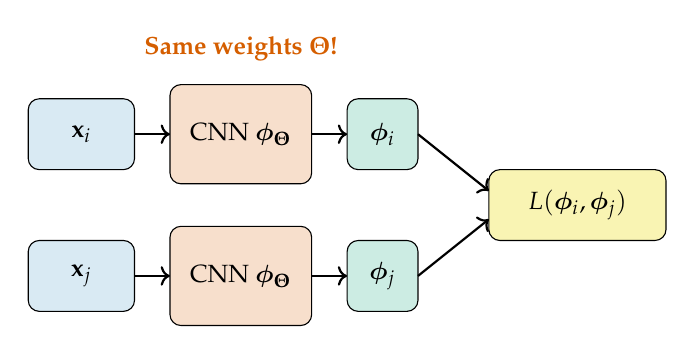
\begin{tikzpicture}[scale=0.9, every node/.style={font=\small}]
    \draw[fill=blue!15, rounded corners] (-3.5, 0.5) rectangle (-2, 1.5);
    \node at (-2.75, 1) {$\vx_i$};
    \draw[fill=red!20, rounded corners] (-1.5, 0.3) rectangle (0.5, 1.7);
    \node at (-0.5, 1) {CNN $\vphi_{\vTheta}$};
    \draw[fill=green!20, rounded corners] (1, 0.5) rectangle (2, 1.5);
    \node at (1.5, 1) {$\vphi_i$};

    \draw[->, thick] (-2, 1) -- (-1.5, 1);
    \draw[->, thick] (0.5, 1) -- (1, 1);

    \draw[fill=blue!15, rounded corners] (-3.5, -1.5) rectangle (-2, -0.5);
    \node at (-2.75, -1) {$\vx_j$};
    \draw[fill=red!20, rounded corners] (-1.5, -1.7) rectangle (0.5, -0.3);
    \node at (-0.5, -1) {CNN $\vphi_{\vTheta}$};
    \draw[fill=green!20, rounded corners] (1, -1.5) rectangle (2, -0.5);
    \node at (1.5, -1) {$\vphi_j$};

    \draw[->, thick] (-2, -1) -- (-1.5, -1);
    \draw[->, thick] (0.5, -1) -- (1, -1);

    \draw[fill=yellow!40, rounded corners] (3, -0.5) rectangle (5.5, 0.5);
    \node at (4.25, 0) {$L(\vphi_i, \vphi_j)$};
    \draw[->, thick] (2, 1) -- (3, 0.2);
    \draw[->, thick] (2, -1) -- (3, -0.2);

    \node[red] at (-0.5, 2.2) {\textbf{Same weights $\vTheta$!}};
\end{tikzpicture}
\end{center}

\vspace{8pt}
\textbf{Loss:} small when $(\vx_i, \vx_j)$ are similar, large when they aren't.

\vspace{4pt}
\textbf{Key feature:} the \emph{same} network processes both inputs. Symmetric by construction.
\end{frame}

\begin{frame}
\frametitle{Triplet Loss}

\textbf{Better idea than ``compatible vs incompatible'' pairs:} use \emph{triples}.

\vspace{6pt}
\textbf{A triplet:} $(a, p, n)$ where
\begin{itemize}
    \item $a$ = anchor.
    \item $p$ = positive (similar to anchor).
    \item $n$ = negative (dissimilar to anchor).
\end{itemize}

\vspace{8pt}
\textbf{Triplet loss:}
\[
    \mathcal{L}(a, p, n) = \max\bigl(0, \;\|\vphi_a - \vphi_p\|^2 - \|\vphi_a - \vphi_n\|^2 + \alpha\bigr)
\]
where $\alpha > 0$ is a margin.

\vspace{6pt}
\textbf{Reading the formula:} push the positive closer and the negative farther by at least $\alpha$.

\vspace{8pt}
\textbf{Where it's used:}
\begin{itemize}
    \item Face recognition (FaceNet, Schroff et al.\ 2015).
    \item Image search (Google Lens).
    \item Speaker recognition.
\end{itemize}

\textcolor{red}{Hard-negative mining is essential -- random negatives are usually too easy.}
\end{frame}

\begin{frame}
\frametitle{Visual Style: Veit et al.\ 2015}

\textbf{Goal:} learn an embedding that captures \emph{compatibility} between clothing items.

\vspace{6pt}
\textbf{Training data:}
\begin{itemize}
    \item $\sim 1$M Amazon products with category labels.
    \item Pairs ``frequently bought together'' = compatible.
    \item Random pairs across categories = incompatible.
\end{itemize}

\vspace{8pt}
\textbf{Architecture:} a Siamese CNN -- two copies of the same conv net producing 128-dim embeddings.

\vspace{6pt}
\textbf{Result:} a learned embedding space where ``items that go together'' cluster, regardless of category.

\vspace{4pt}
A red T-shirt and a blue T-shirt are near each other; a red T-shirt and a leather belt are near each other; but a red T-shirt and a dress are far.

\vspace{4pt}
\textcolor{blue}{This is the canonical industry use case -- it's how Amazon shopping recommendations work.}
\end{frame}

\begin{frame}
\frametitle{Modern Context: Contrastive Learning}

\textbf{Triplet loss generalizes to many forms of contrastive learning.}

\vspace{6pt}
\textbf{SimCLR, MoCo, DINO} (2020s) for images:
\begin{itemize}
    \item For each image, two augmented views = positive pair.
    \item Every other image in the batch = negative.
    \item Train the encoder so positives are close, negatives are far.
\end{itemize}

\vspace{8pt}
\textbf{CLIP} (Radford et al., 2021):
\begin{itemize}
    \item Image-text dual encoder.
    \item Caption matches its image; other captions are negatives.
    \item The shared embedding space lets you do zero-shot classification.
\end{itemize}

\vspace{8pt}
\textbf{SBERT} (Reimers \& Gurevych, 2019):
\begin{itemize}
    \item Sentence-level Siamese BERT for semantic similarity.
\end{itemize}

\vspace{4pt}
\textcolor{red}{All of these are direct descendants of the Siamese / triplet idea from the early 2010s.}
\end{frame}

\begin{frame}
\frametitle{Section Summary}

\textbf{From lookup to neural:}
\begin{itemize}
    \item Lookup embeddings: $\vu_s = \vE[s, :]$. Stored, not computed.
    \item Deep embeddings: $\vu_s = \vphi_{\vTheta}(\vx_s)$. Computed from features.
\end{itemize}

\vspace{6pt}
\textbf{Training paradigms:}
\begin{itemize}
    \item Siamese networks: pair-based loss with shared weights.
    \item Triplet loss: anchor + positive + negative with a margin.
    \item Contrastive learning: many negatives per positive (SimCLR, CLIP, DINO).
\end{itemize}

\vspace{8pt}
\textcolor{red}{All modern representation learning lives in this family.}

\vspace{6pt}
\textbf{Coming up:} a critical limitation of everything we've seen so far -- the embeddings are \emph{static}.
\end{frame}


% ============================================================
\section{Static vs Contextual Embeddings}
% ============================================================

\begin{transitionframe}
\begin{center}
{\Huge \textbf{Static vs Contextual Embeddings}}\\[10pt]
{\large The limit of word2vec}
\end{center}
\end{transitionframe}

\begin{frame}
\frametitle{The Problem with Static Embeddings}

\textbf{Static embedding:} each word has \emph{one} vector, no matter the sentence.

\vspace{8pt}
\textbf{The classic example:}

\vspace{4pt}
\begin{itemize}
    \item ``I deposited my paycheck at the \textcolor{blue}{\textbf{bank}}.''
    \item ``The boat drifted to the river \textcolor{blue}{\textbf{bank}}.''
\end{itemize}

\vspace{6pt}
Both occurrences of \textit{bank} get \emph{the same vector} from word2vec.

\vspace{8pt}
\textbf{Worse, for econ:}
\begin{itemize}
    \item ``The Fed hiked the \textbf{rate}.'' (interest rate)
    \item ``This is a high-\textbf{rate} of inflation.'' (rate as ratio)
    \item ``Rate the product 1--5 stars.'' (rate as verb)
\end{itemize}

\vspace{4pt}
\textcolor{red}{Three different meanings, one vector. Word2vec averages them all.}
\end{frame}

\begin{frame}
\frametitle{What We Want: Context-Dependent Vectors}

\textbf{The fix:} make the embedding of a word depend on its surrounding sentence.
\[
    \vu_{\text{bank}} \;\longrightarrow\; \vu_{\text{bank}}(\text{context})
\]

\vspace{8pt}
\textbf{Two consequences:}
\begin{itemize}
    \item Different occurrences of the same word can have different vectors.
    \item The same word in different sentences can land in different parts of embedding space.
\end{itemize}

\vspace{8pt}
\textbf{Three generations of solutions:}
\begin{enumerate}
    \item \textbf{ELMo} (2018): bidirectional LSTM produces context-dependent vectors.
    \item \textbf{BERT} (2018): transformer encoder, contextual at every layer.
    \item \textbf{GPT, LLaMA, modern LLMs}: causal transformers, contextual everywhere.
\end{enumerate}

\vspace{6pt}
\textcolor{red}{All three rely on the \emph{attention} mechanism -- the topic of next class.}
\end{frame}

\begin{frame}
\frametitle{What Attention Will Do for Us}

\textbf{Preview} (full treatment next lecture):

\vspace{6pt}
For each word in a sentence, compute its embedding as a \emph{weighted average} of \emph{all other words}' embeddings.

\vspace{4pt}
The weights depend on how relevant each other word is.

\vspace{8pt}
\begin{tikzpicture}
\node [mybox] (box){%
    \begin{minipage}{0.9\textwidth}
    \vspace{-4pt}
    \[
        \vu_i \;=\; \sum_{j=1}^T \alpha_{ij} \vv_j
        \quad\text{where}\quad
        \alpha_{ij} = \frac{\exp(\vq_i^\top \vk_j)}{\sum_l \exp(\vq_i^\top \vk_l)}
    \]
    \vspace{-12pt}\\[-2pt]
    Each word $i$ \emph{looks at} every word $j$ in the sentence with attention weight $\alpha_{ij}$.
    \end{minipage}
};
\node[fancytitle, right=10pt] at (box.north west) {Sneak peek: self-attention};
\end{tikzpicture}

\vspace{8pt}
\textbf{Result:} the embedding of \textit{bank} in ``river bank'' attends strongly to \textit{river}; in ``paycheck at the bank'' it attends to \textit{paycheck}.

\vspace{4pt}
\textcolor{blue}{Same word, different vectors -- because the context is different.}
\end{frame}

\begin{frame}
\frametitle{Why It Matters for Economics}

\textbf{Static embeddings} (word2vec, GloVe):
\begin{itemize}
    \item Cheap to compute, easy to share.
    \item Useful for clustering or simple regression features.
    \item Limitation: polysemy + lack of context.
\end{itemize}

\vspace{8pt}
\textbf{Contextual embeddings} (BERT, GPT, modern):
\begin{itemize}
    \item Same word can mean different things in different sentences.
    \item Capture fine-grained semantics: ``\textbf{tasa} de inter\'es'' vs ``\textbf{tasa} de mortalidad''.
    \item Required for nuanced sentiment, stance detection, narrative analysis.
\end{itemize}

\vspace{8pt}
\textbf{For your work:}
\begin{itemize}
    \item Use \texttt{sentence-transformers} (SBERT, Spanish models like \texttt{beto}) over word2vec for FOMC / BCRP analysis.
    \item Treat word2vec as a baseline; modern contextual models give noticeably better accuracy on sentiment and topic tasks.
\end{itemize}

\vspace{4pt}
\textcolor{red}{We'll see how this works under the hood next class.}
\end{frame}


% ============================================================
\section{Summary and Next Steps}
% ============================================================

\begin{transitionframe}
\begin{center}
{\Huge \textbf{Summary \& Next Steps}}
\end{center}
\end{transitionframe}

\begin{frame}
\frametitle{Key Takeaways}

\textbf{Technical highlights of today:}

\vspace{6pt}
\begin{enumerate}
    \item \textbf{Embeddings} represent objects as vectors where geometry captures useful relationships.

    \vspace{4pt}
    \item \textbf{LLE} preserves local linear reconstruction weights from high dim to low dim, via the matrix $\vM = (\mathbf{I} - \vW)^\top (\mathbf{I} - \vW)$.

    \vspace{4pt}
    \item \textbf{Word2vec} learns embeddings by predicting context words from center words; objective is the average log-likelihood over a sliding window.

    \vspace{4pt}
    \item \textbf{Skip-gram softmax} costs $O(W D)$ per training pair -- prohibitive at $W \sim 10^5$.

    \vspace{4pt}
    \item \textbf{Hierarchical softmax} replaces one $W$-way decision with a path of binary decisions: $O(\log_2 W \cdot D)$ per pair.

    \vspace{4pt}
    \item \textbf{Huffman trees} make frequent words cheaper by assigning them shorter paths -- expected length below balanced for Zipfian data.

    \vspace{4pt}
    \item \textbf{Negative sampling} is the modern alternative: $O(k D)$ per pair, simpler to implement, default in practice.
\end{enumerate}
\end{frame}

\begin{frame}
\frametitle{Today's Big Ideas}

\begin{enumerate}
    \item \textbf{Embedding} = learned vector representation of a discrete object.

    \vspace{4pt}
    \item \textbf{Two geometries:} distance encodes clustering; inner product encodes direction (and is exactly a latent factor model).

    \vspace{4pt}
    \item \textbf{Word2vec} = skip-gram + negative sampling. Levy-Goldberg: it's matrix factorization of shifted PMI.

    \vspace{4pt}
    \item \textbf{Vector arithmetic} captures linguistic regularities -- not magic, just linear structure.

    \vspace{4pt}
    \item \textbf{For economics:} embed firms, judges, countries, central bank text. Use as features for downstream analysis.

    \vspace{4pt}
    \item \textbf{Deep embeddings:} replace lookup with a neural network. Siamese, triplet, contrastive -- all variants of the same idea.

    \vspace{4pt}
    \item \textbf{Static $\to$ contextual} is the next frontier. Attention is the mechanism.
\end{enumerate}
\end{frame}

\begin{frame}
\frametitle{The Big Picture}

\begin{center}
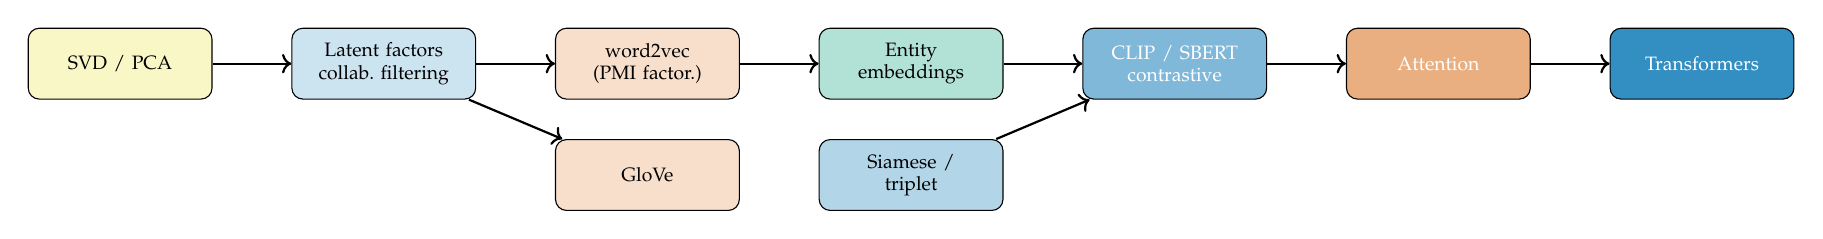
\begin{tikzpicture}[node distance=0.5cm and 1cm, every node/.style={draw, rounded corners, align=center, font=\scriptsize, minimum height=0.9cm, text width=2.1cm}]
    \node (svd) [fill=yellow!30] {SVD / PCA};
    \node (lfm) [right=of svd, fill=blue!20] {Latent factors \\ collab.\ filtering};
    \node (w2v) [right=of lfm, fill=red!20] {word2vec \\ \scriptsize (PMI factor.)};
    \node (glove) [below=of w2v, fill=red!20] {GloVe};
    \node (ent) [right=of w2v, fill=green!30] {Entity \\ embeddings};
    \node (siam) [below=of ent, fill=blue!30] {Siamese / \\ triplet};
    \node (clip) [right=of ent, fill=blue!50, text=white] {CLIP / SBERT \\ \scriptsize contrastive};
    \node (att) [right=of clip, fill=red!50, text=white] {Attention};
    \node (tr) [right=of att, fill=blue!80, text=white] {Transformers};

    \draw[->, thick] (svd) -- (lfm);
    \draw[->, thick] (lfm) -- (w2v);
    \draw[->, thick] (lfm) -- (glove);
    \draw[->, thick] (w2v) -- (ent);
    \draw[->, thick] (ent) -- (clip);
    \draw[->, thick] (siam) -- (clip);
    \draw[->, thick] (clip) -- (att);
    \draw[->, thick] (att) -- (tr);
\end{tikzpicture}
\end{center}

\vspace{12pt}
\textbf{Reading the diagram:}
\begin{itemize}
    \item Yellow = Lecture 6 (linear factor methods).
    \item Red = today's content.
    \item Blue / white = where we're going.
\end{itemize}

\vspace{4pt}
\textcolor{red}{Each box is the previous box's loss function applied to a new type of data, or a new architecture replacing the linear lookup.}
\end{frame}

\begin{frame}
\frametitle{Practical Recipes}

\textbf{When to use what:}
\begin{itemize}
    \item Need a quick embedding from your own corpus $\to$ \textbf{word2vec} or \textbf{GloVe}.
    \item Need state-of-the-art Spanish embeddings $\to$ \textbf{BETO, RoBERTa-es, sentence-transformers}.
    \item Embedding new entities (firms, countries, judges) $\to$ \textbf{custom skip-gram} on your co-occurrence signal.
    \item Image / multimodal embeddings $\to$ \textbf{CLIP, DINOv2, BLIP}.
    \item Visualization $\to$ \textbf{t-SNE} (small data), \textbf{UMAP} (large), \textbf{PCA} (reproducible).
\end{itemize}

\vspace{8pt}
\textbf{Common pitfalls:}
\begin{itemize}
    \item Don't use t-SNE / UMAP coordinates as features -- they're for visualization only.
    \item Don't trust word2vec analogies blindly; check sample size and corpus quality.
    \item Don't forget that embeddings are estimated; downstream standard errors should account for that.
\end{itemize}
\end{frame}

\begin{frame}
\frametitle{Next Lecture: Attention and Self-Attention}

\textbf{Lecture 8:}
\begin{itemize}
    \item The attention mechanism: queries, keys, values.
    \item Self-attention: a sentence attends to itself.
    \item Multi-head attention: multiple ``views'' of the same sequence.
    \item Foundation for the Transformer (Lecture 9).
\end{itemize}

\vspace{8pt}
\textbf{The transition:} we move from \emph{static} lookup tables (today) to \emph{dynamic} context-dependent embeddings (next class).

\vspace{8pt}
\textbf{Recommended reading:}
\begin{itemize}
    \item Mikolov et al.\ (2013), \emph{Distributed representations of words and phrases}.
    \item Levy \& Goldberg (2014), \emph{Neural word embedding as implicit matrix factorization}.
    \item Gentzkow, Kelly \& Taddy (2019), \emph{Text as data}, JEL.
    \item Vaswani et al.\ (2017), \emph{Attention is all you need} (prep for next class).
\end{itemize}

\vspace{6pt}
\begin{center}
\Large \textcolor{blue}{\textbf{Questions?}}
\end{center}
\end{frame}

\begin{frame}
\frametitle{References}

\footnotesize
\begin{itemize}
    \item Roweis, S., \& Saul, L. (2000). Nonlinear dimensionality reduction by locally linear embedding. \textit{Science}, 290.
    \item van der Maaten, L., \& Hinton, G. (2008). Visualizing data using t-SNE. \textit{JMLR}, 9.
    \item McInnes, L., Healy, J., \& Melville, J. (2018). UMAP: uniform manifold approximation and projection.
    \item Mikolov, T., Sutskever, I., Chen, K., Corrado, G., \& Dean, J. (2013). Distributed representations of words and phrases. \textit{NIPS}.
    \item Pennington, J., Socher, R., \& Manning, C. (2014). GloVe: global vectors for word representation. \textit{EMNLP}.
    \item Levy, O., \& Goldberg, Y. (2014). Neural word embedding as implicit matrix factorization. \textit{NIPS}.
    \item Schroff, F., Kalenichenko, D., \& Philbin, J. (2015). FaceNet: a unified embedding for face recognition. \textit{CVPR}.
    \item Veit, A., Kovacs, B., Bell, S., McAuley, J., Bala, K., \& Belongie, S. (2015). Learning visual clothing style with heterogeneous dyadic co-occurrences. \textit{ICCV}.
    \item Radford, A., et al. (2021). Learning transferable visual models from natural language supervision (CLIP). \textit{ICML}.
    \item Reimers, N., \& Gurevych, I. (2019). Sentence-BERT: sentence embeddings using Siamese BERT. \textit{EMNLP}.
    \item Hansen, S., \& McMahon, M. (2016). Shocking language: understanding the macro effects of central bank communication. \textit{JIE}.
    \item Hoberg, G., \& Phillips, G. (2016). Text-based network industries and endogenous product differentiation. \textit{JPE}.
    \item Gentzkow, M., Kelly, B., \& Taddy, M. (2019). Text as data. \textit{JEL}, 57(3).
    \item Ash, E., \& Chen, D. (2023). Case vectors: spatial representations of the law. (Working paper series on judge embeddings.)
\end{itemize}
\end{frame}


\end{document}
